\section{Methods}

\begin{figure}[t]
\centering
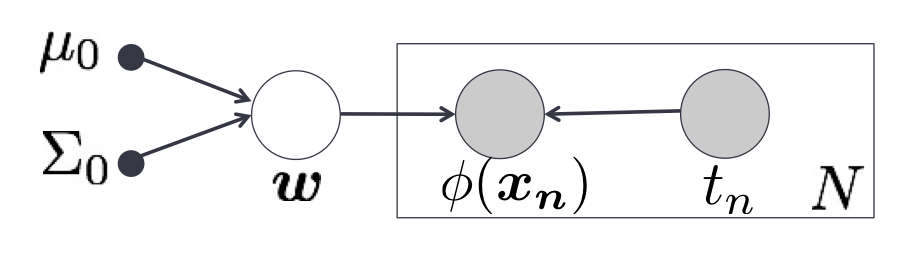
\includegraphics[height=3.0cm]{BLR_graphical.png}

\caption{\small Graphical model of Bayesian logistic regression. Here
$t_n \in \{0,1\}$ is the class label, $\phi({\bf x}_n)$ is the feature map,
and ${\bf w}$ is the model parameter.}

\label{fig:BLR_graphical}
\end{figure}

Given data set $\{\phib_n, t_n\}_{n=1}^N$ where $\phib_n$ are the feature
vectors and $t_n\in \{0,1\}$ are the labels, we can write the likelihood
function for logistic regression as $p(\bm{t}|\bm{w}) = \prod_{n=1}^N
y_n^{t_n} (1-y_n)^{1-t_n}$ where $\bm{t} = (t_1,...,t_N)^T$ and
$y_n=p(\mathcal{C}_1|\phib_n) = \sigma(\bm{w}^T \phib_n)$ and $\sigma(s) =
\frac{1}{1+e^{-s}}$. Using Bayes rule, the posterior distribution over
$\bm{w}$ is $p(\bm{w}|\bm{t}) = \frac{p(\bm{w}) p(\bm{t}|\bm{w})}{p(\bm{t})}$
where $p(\bm{t}) = \int p(\bm{w})p(\bm{t}|\bm{w}) d\bm{w}$ involves logistic
sigmoid functions and is intractable. In the sequel we briefly describe three
approximation schemes (Laplace approximation, variational methods, and Gibbs
sampling), and point estimations (MLE, MAP) together with the associated
prediction rules.

\subsection{Markov Chain Monte Carlo approximation}
\label{sec:MCMCmethod}
Let us first discuss the simple bayesian binary probit regression model and 
then we will ease into bayesian logistic regression. We follow the lead of
the work done by Holmes et al.~\cite{Holmes}. Let $\psi$ denotes the gaussian
cdf, binary probit regression's likelihood is:
\begin{equation}
\pi(y_i=1|x_i) = \psi(x_i^Tw)
\end{equation}

We define a set of n auxiliary variables $z_i$ as there is no cojugate prior to
the gaussian cdf as:
\begin{equation}
z_i=x_i^Tw+\epsilon_i
\end{equation}

and $\epsilon_i \sim N(0,1)$, and if $z_i>0$ then $y_i=1$ and vice-versa.
Removing w from likelihood in this new model makes the model more amenable
to sampling. For this
specific case of  Normal prior over w, this model has a simple
Gibbs sampling updates where $z_i$ is drawn from independent 
truncated Normal distributions, and w is drwn from a multvariate Normal
distribution. Formally, a easy-to-follow Gibbs sampling scheme with
$\pi(w)\sim N(b,v)$ can be obtained using the following:
\begin{eqnarray}
z_i|w \propto N(x_i^Tw,1)I(z_i>0)y_i=1 \\
z_i|w \propto N(x_i^Tw,1)I(z_i\leq 0)y_i\neq 0 \\
w|z,y \sim N(B,V) \\
B = V(v^{-1}b+X^Tz) \\
V=(v^{-1}+X^TX)^-1 \\
\end{eqnarray}

This simple Gibbs sampling strategy is poor in performance because the
components of w are strongly correlated with the components of z. To remove this
we sample w and z together through the use of the product rule:
\begin{equation}
\pi(w,z|y) = \pi(z|y)*\pi(w|z)
\end{equation}

This method draws every $z_i$ from a Normal distribution that has means
and variances obtained using a leave-one-out marginal predictive density,
and these conditional means are updated after each draw of $z_i$.
Later we sample w from its conditional gaussian after all of the
$z_i$ have been drawn. 



\subsubsection{Binary Logistic Regression}
Starting from the binary Bayesian probit regression model explained before , we
propose to obtain updates for binary Bayesian logistic regression by
substituting the independent Normal 
prior over $\epsilon$ with independent logistic. 
This significantly alters the simple sampling scheme we described earlier. To
obtain a simple sampling strategy of the new model we define an addtional group
of auxiliary variables $λ_{1:n}$ along side modifying the noise function to get
a scale mixture of gaussians with marginal densities as logistic distribution,
(here KS is the Kolmogorov-Smirnov distribution):
\begin{eqnarray}
\epsilon_i \sim N(0,\lambda_i) \\
\lambda_i = (2\nu_i)^2 \\
\nu_i \sim KS \\
\end{eqnarray}

If one takes $\lambda$ to be  constant, then this is identical to the
Probit model above. Though each value of $z_i$ contains an individual term i for
its noise variance now. Moreover, the greatest advantage is that we know the way
to draw samples from this model given fixed $\lambda$ . We just have to use
weighted least squares rather than least squares (and teh related inverse of the 
hessian matrix), and then just draw from individual truncated gaussain of
different variance parameters. After this, we are in a poition to write a
Gibbs sampler given that we will be able to sample from the KS distribution.
\cite{Holmes} provides rejection sampling technique to draw samples 
from the KS distribution via the Generalized Inverse Gaussian distibution as the
sampling density. Using this, we write a simple Gibbs sampler for this
logistic regression setting as follows:

\begin{eqnarray}
z_i|w,\lambda \propto N(x_i^Tw,\lambda_i)I(z_i>0)~if~y_i=1 \\
z_i|w,\lambda \propto N(x_i^Tw,\lambda_i)I(z_i\leq 0)~if~y_i\neq 0 \\
w|z,y.\lambda \sim N(B,V) \\
B = V(v^{-1}b+X^TWz) \\
V=(v^{-1}+X^TWX)^{-1} \\
W=diag(\lambda^{-1}) \\
\end{eqnarray}

We use block Gibbs sampling here. 
There are two approaches to performing block sampling of the parameters above.
In the first approach we sample $z$ and $w$ simultaneously and the parameter
$\lambda$ is sampled after that. In the second approach 
the block sampling updates $z$ and
$\lambda$ first and $z$ later. This way the $z_i|w,\lambda$ follows a
truncated logistic centered at $x_i^Tw$. This avoids the need to compute
marginal predictive densities.    

Another way to sample Bayesian Logistic Regression is via the use of uniform
distribution. Groenewald et al.~\cite{Groenewald2005} provide a scheme to
use uniform distribution for such a task. As we know 
\begin{equation}
\pi_i = \frac{exp(x_i^Tw)}{1+exp(x_i^Tw)}
\end{equation} 
The equation above can also be written as a CDF of a uniform distribution as
follows:
\begin{equation}
\pi_i = \int_{-\infty}^{x_i^Tw} \frac{exp(z)}{1+exp(z)} \partial z =
P(U<\frac{exp(x_i^Tw)}{1+exp(x_i^Tw)})
\label{eqn:uniformSample}
\end{equation}

Here we have cleverly introduced an auxiliary variable $U$.
Now a gibbs sampler can easly be derived which alternates between $w$ and $u$.
Though it sounds enticing the sampler obtained using this technique is high
degree of auto-correlation between $w$ and $u$ and converges very poorly in all
our experiments. Figure~\ref{fig:uniformSamplerChain} shows a typical uniform
distribution based sampler on our datasets. The chain rarely converges with very
poor results. We abandon the discussion of this method here and
concentrate only on Kolmogorov Smirnov based sampling in the later sections.

\begin{figure}[t]
\label{fig:laplace}
\centering
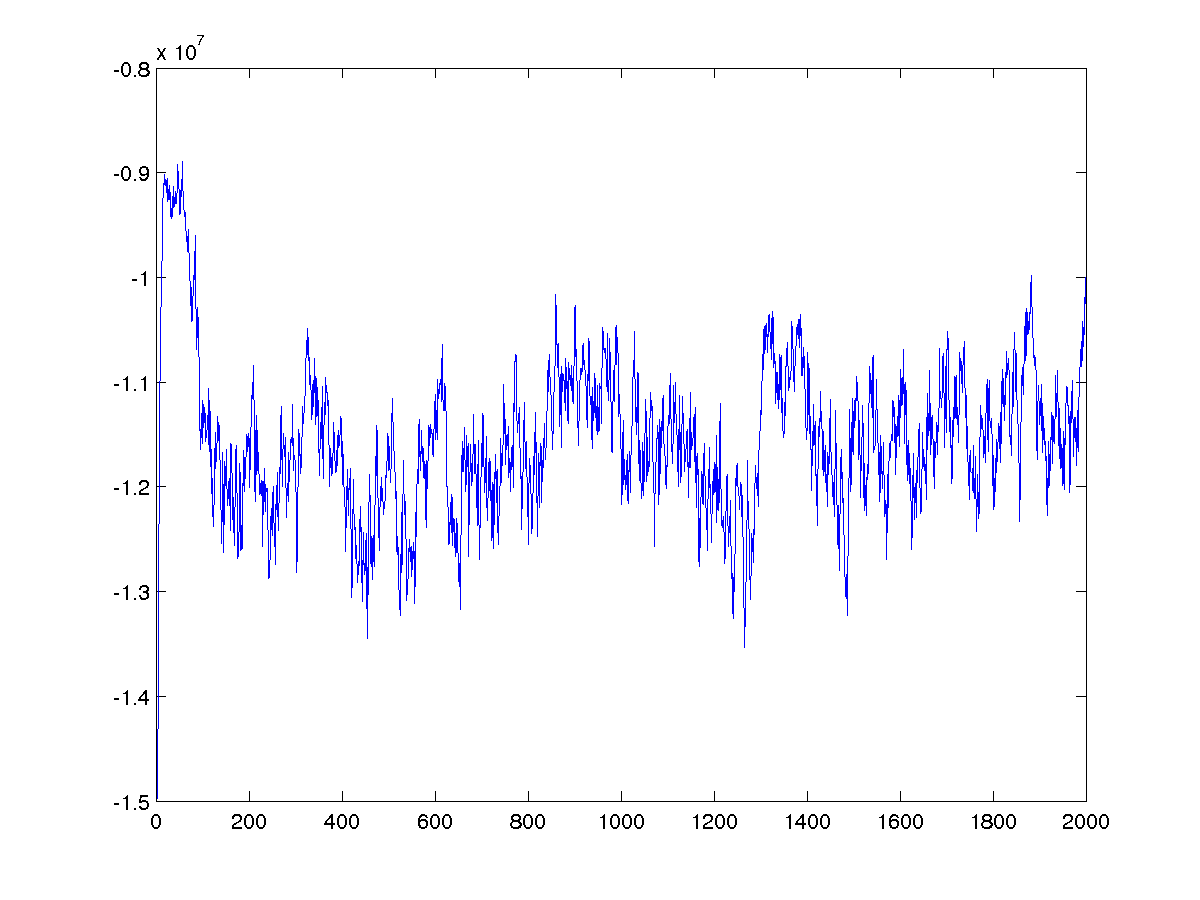
\includegraphics[height=10.0cm]{results/uniformSampleChain.png}

\caption{A typical Markov chain for uniform distribution based sampler on the
Spambase dataset}

\label{fig:uniformSamplerChain}
\end{figure}




\subsection{Laplace Approximation and associated MAP}

Laplace approximation approximate the posterior $p(\bm{w}|\bm{t})$ with a
multivariate Guassian $\mathcal{N}(\bm{w}; \bm{w}_{MAP},\Sigma_N)$ where
$\wb_{MAP}$ is the maximum {\it a posteriori} and thus a mode of the
posterior and $\Sigma_N^{-1} = -\nabla^2_{\bm{w}} \ln
p(\bm{w}|\bm{t})|_{\bm{w} = \bm{w}_{MAP}}$ is the Hessian at $\bm{w}_{MAP}$.
Since we are approximating the posterior with Gaussian, it is convenient to
use conjugate prior $p(\bm{w}) = \mathcal{N}(\bm{w};\bm{m}_0,\Sigma_0)$. Thus
we have
\begin{equation}
\ln p(\bm{w}|\bm{t}) = -\frac{1}{2}(\bm{w}-\bm{m}_0)^T
\Sigma_0^{-1}(\bm{w}-\bm{m}_0) + \sum_{n=1}^N\{t_n \ln y_n +(1-y_n) \ln
(1-y_n)\} + const
\end{equation}

Under the Laplace approximation and the conjugated Gaussian prior, $\bm{w}_{MAP}$
can be efficiently obtained by gradient descent. To encourage small
$||w||^2_2$, let $\bm{m}_0 = \bm{0}$, and $\Sigma_0 = \sigma^2 \bm{I}$, we
have the following gradient descent rule: 

\begin{equation}
\bm{w}_t \leftarrow \bm{w}_{t-1} + \eta\left( \sum_{n=1}^N (t_n - y_{n,(t-1)}) \phib_n -
\frac{1}{\sigma^2}\bm{w}_{t-1} \right)
\end{equation}

where $\eta$ is the learning rate constant. We can also get

\begin{equation}
\Sigma_N^{-1} = -\nabla^2_{\bm{w}} \ln p(\bm{w}|\bm{t})
= \Sigma_0^{-1} + \sum_{n=1}^N y_n(1-y_n) \phib_n \phib_n^T
\end{equation}

The predictive distribution for Laplace-approximated posterior is not close
form, but by approximating the logistic sigmoid function with probit function,
we recover $\bm{w}_{MAP}$ as the decision boundary.



\subsection{The Variational Approach by Jaakkola and Jordan}
We study a variational method presented by Jaakkola et al.\cite{Jaakkola96avariational}. In this section, we briefly describe this variational approach for approximate inference for Bayesian logistic regression. 

Since it is infeasible to compute the posterior $p(\bm{w} | \bm{t}, \bm{\phi})$ exactly, this method approximates the sigmoid function with its variational form, as given below.

\begin{align}
  p(t | \bm{w}, \phi) &= \sigma(\Phi_s) \geq \sigma(\xi) exp\{(Phi_s - \xi)/2 + \lambda(\xi)(\Phi_s^2 - \xi^2)\} \\
  &= P(t | \bm{w}, \phi, \xi)
\end{align}
where $\Phi_s = (2t - 1)\sum_jw_j\phi_j$ and $\lambda(\xi) = [1/2 - \sigma(\xi)]/(2\xi)$.

The posterior $P(\bm{w}|\bm{t}, \bm{\phi})$ can be computed by normalizing the left hand side of the following equation.
\begin{align}
\label{eq:variational}
p(\bm{t}|\bm{\phi})p(\bm{w}) &\geq P(\bm{t}|\bm{\phi}, \bm{w}, \xi)P(\bm{w})
\end{align}

Since this normalization is not feasible in practice we normalize the variational distribution instead. As the prior distribution is a Gaussian, we assume it has mean $\mu$ and covariance matrix $\Sigma$. To compute the variational posterior, first, we absorb the observations to update $\mu$ and $\Sigma$.

For each observation, $Sigma$ and $\mu$ are updated as below: 
\begin{align}
\label{eq:sigma_update}
\Sigma^{-1}_{post} &= \Sigma^{-1} + 2|\lambda(\xi)|\phi\phi^T\\
\label{eq:mu_update}
\mu_{post} &= \Sigma_{post}[\Sigma^{-1}\mu + (t - 1/2)\phi]
\end{align}
where $\phi = [\phi_1 ...\phi_n]^T$. 

Now, the posterior covariance matrix depends on the variational parameter $\xi$ through $\lambda(\xi)$ and thus its value needs to be obtained. We obtain $\xi$ by optimizing the approximation in eq. (\ref{eq:variational}). A fast EM algorithm is devised to perform this optimization. This leads to a closed form update for $\xi$. For each observation, the update equation is given by 
\begin{align}
\label{eq:xi}
\xi^2 = E\{(\sum_jw_j\phi_j)^2\} &= \phi^T\Sigma_{post}\phi + (\phi^T\mu_{post})^2
\end{align}

where the expectation is taken with respect to $P(\bm{w}|\bm{\phi}, \xi^{old})$, the variational posterior distribution based on the previous vaue of $\xi$. Alternating between eq. (\ref{eq:sigma_update}), eq. (\ref{eq:mu_update}) and eq. (\ref{eq:xi}) monotonically improves the posterior approximation of eq. (\ref{eq:variational}).

Let $\mathcal{D}$ be the set of all observations. The predictive likelihoods $P(t^p | w_p, \mathcal{D})$ for any complete observation $D^t$ is given by
\begin{align}
  logP(t^p|w_p, \mathcal{D}) = log(\xi_p) - \xi_p/2 - \lambda(\xi_p)\xi_p^2 - \frac{1}{2}\mu^T\Sigma^{-1}\mu + \frac{1}{2}\mu^T_t\Sigma^{-1}_t\mu_t + \frac{1}{2}log\frac{|\Sigma_t|}{|\Sigma|}
\end{align}
where $\mu$ and $\Sigma$ signify the parameters in $P(\bm{w})$ and the subscript $p$ refers to the posterior $P(\bm{w}|\mathcal{D}, D^p)$ found by absorbing the evidence in $D^p$.

We implemented this algorithm, mainly the updating rules in eq. (\ref{eq:sigma_update}), eq. (\ref{eq:mu_update}) and eq. (\ref{eq:xi}). The main advantage of this algorithm is that it usually converges in only 2 to 3 iterations. Although the computation involves expensive matrix inversion, matrix inversion here can be computed as solving a linear system. Therefore, this approach is still pretty fast.

\subsection{Delta Method}


